% !TeX program = pdflatex
%==============================================================================
%  Aula 07 --- Pré-processamento e Pipelines
%  VERSÃO DO ALUNO: texto para leitura autônoma, fora da sala.
%  (O roteiro de sala é "07 Pre-processamento e Pipelines.tex".)
%==============================================================================
\documentclass[11pt,a4paper]{article}
\usepackage[aluno]{../../recursos/latex/estilo-notas}

\title{}
\date{}

\begin{document}
\cabecalhoaula{07}{Pré-processamento e \emph{Pipelines}}{ISLP labs cap.~5--6; AME §2.1.2}

%==============================================================================
\section*{O que você vai aprender}
%==============================================================================
Ao final desta aula você deve ser capaz de:
\begin{itemize}[leftmargin=1.4cm]
  \item explicar por que o pré-processamento faz parte do \emph{modelo}, e não dos
        dados;
  \item definir a \textbf{padronização} (\texttt{StandardScaler}) e listar suas
        vantagens e desvantagens;
  \item identificar e evitar o \textbf{vazamento de dados} (\emph{data leakage}),
        e saber \emph{quais} vazamentos são graves;
  \item construir um \textbf{\emph{pipeline}} que encadeia pré-processamento e
        estimador como um único objeto;
  \item combinar \emph{pipeline} com validação cruzada e busca de hiperparâmetros
        sem vazamento;
  \item conhecer outros pré-processamentos comuns (imputação, codificação de
        categóricas) e o \texttt{ColumnTransformer}.
\end{itemize}

\noindent
Esta é a aula que costura as anteriores em \emph{boas práticas de implementação}.
Vários métodos já exigiram padronização --- Lasso e Ridge (Aula~02), KNN
(Aula~04) --- e a Aula~03 já avisou sobre vazamento. Aqui formalizamos \emph{como}
fazer isso certo. Comece pela pergunta:

\begin{center}\itshape
  onde, exatamente, eu devo calcular a média e o desvio para padronizar:\\
  antes ou depois de separar treino e teste?
\end{center}

\noindent
A resposta canônica é ``depois'', e você vai vê-la justificada na
Seção~\ref{sec:vazamento}. Mas a Figura~\ref{fig:vazamento} vai mostrar que,
\emph{nesse caso específico}, a diferença é praticamente nula --- e que o vazamento
que realmente destrói uma análise é outro. Vale ler até lá antes de tirar conclusões.

%==============================================================================
\section{Motivação: o pré-processamento é parte do modelo}
%==============================================================================
Na prática, raramente alimentamos o estimador com os dados brutos. Um fluxo típico
encadeia várias transformações: padronizar, imputar faltantes, codificar variáveis
categóricas, reduzir dimensão (PCA), e só então ajustar o modelo. A tentação é
aplicar essas transformações ``de uma vez'' no conjunto inteiro --- e é exatamente aí
que mora o erro.

\begin{ideia}
O insight central da aula: \textbf{toda transformação que ``aprende'' algo dos
dados} (uma média, um desvio, as categorias presentes, os componentes principais)
é \emph{parte do procedimento de estimação}. Logo, deve ser \emph{ajustada apenas
no treino} e \emph{aplicada} ao teste/validação --- nunca o contrário.
\end{ideia}

\noindent
Um teste mental que resolve quase todos os casos: pergunte-se \emph{``essa etapa
usa os dados para decidir alguma coisa?''}. Tomar o logaritmo de uma coluna,
não --- é a mesma função para qualquer conjunto. Subtrair a média, sim. Escolher
as 20 variáveis mais correlacionadas com $y$, sim, e muito. Quanto mais a etapa
``olha'' para os dados, mais ela pertence ao modelo.

%==============================================================================
\section{O \texttt{StandardScaler} (padronização)}
%==============================================================================
Cada coluna $\bm{X}_i$ de uma base é uma amostra de uma variável aleatória $X_i$ com
$\mu_i=\E[X_i]$ e $\sigma_i^2=\Var(X_i)$ (supostos finitos). A \textbf{padronização}
transforma
\begin{equation}\label{eq:std}
  \widetilde{X}_i = \frac{X_i - \mu_i}{\sigma_i},
\end{equation}
de modo que cada covariável passa a ter média $0$ e variância $1$. Na prática,
$\mu_i$ e $\sigma_i$ são desconhecidos e \emph{estimados} pela média e desvio
amostrais --- e é justamente esse ``estimados'' que cria o risco de vazamento.

\subsection{Vantagens}
\begin{itemize}[leftmargin=1.4cm,nosep]
  \item Covariáveis tornam-se \textbf{adimensionais}: somem as unidades (kg, R\$,
        anos).
  \item Resolve \textbf{discrepâncias numéricas} entre escalas --- crucial para
        métodos baseados em distância (KNN, Aula~04) e em penalização
        (Lasso/Ridge, Aula~02), que de outro modo seriam dominados pelas variáveis
        de maior magnitude.
  \item Torna o \textbf{intercepto desnecessário} em regressão linear (dados
        centrados em zero).
\end{itemize}

\subsection{Desvantagens}
\begin{itemize}[leftmargin=1.4cm,nosep]
  \item Leve perda de \textbf{interpretabilidade}: os coeficientes passam a estar
        em ``desvios-padrão'', não nas unidades originais.
  \item $\mu_i$ e $\sigma_i$ são \textbf{aprendidos dos dados} --- exigindo
        cuidado para não vazar informação do teste (próxima seção).
\end{itemize}

\begin{atencao}
Nem todo método precisa de padronização. Árvores, florestas e \emph{boosting}
(Aula~06) comparam valores \emph{dentro} de cada variável e são completamente
indiferentes à escala --- padronizar não muda nada além de gastar tempo. Já KNN e
qualquer coisa penalizada precisam. Saber \emph{por que} cada método precisa (ou
não) é melhor do que padronizar por reflexo.
\end{atencao}

%==============================================================================
\section{Vazamento de dados (\emph{data leakage})}\label{sec:vazamento}
%==============================================================================
\begin{atencao}[A armadilha]
Se você aplicar o \texttt{StandardScaler} (ou qualquer transformação que aprende
parâmetros) no \emph{conjunto inteiro antes} de separar treino e teste, a
média/desvio usados no treino \textbf{já contêm informação do teste}. As métricas
deixam de medir o desempenho em dados \emph{verdadeiramente novos} e ficam
otimistas. Isso é \textbf{vazamento de dados}.
\end{atencao}

A regra correta:
\begin{enumerate}[leftmargin=1.6cm,nosep]
  \item separe treino e teste \emph{primeiro};
  \item \texttt{fit} do scaler \textbf{só no treino} (aprende $\widehat\mu$,
        $\widehat\sigma$ do treino);
  \item \texttt{transform} aplicado ao treino \emph{e} ao teste com \emph{esses
        mesmos} parâmetros.
\end{enumerate}
O mesmo vale para \emph{cada dobra} da validação cruzada (Aula~03): o scaler deve
ser reajustado usando apenas o treino \emph{daquela} dobra.

\subsection{Quanto custa vazar? Duas medições}
Essa recomendação costuma ser repetida sem número nenhum. Vale medir, e o resultado
tem uma surpresa (Figura~\ref{fig:vazamento}).

\begin{figure}[htbp]
  \centering
  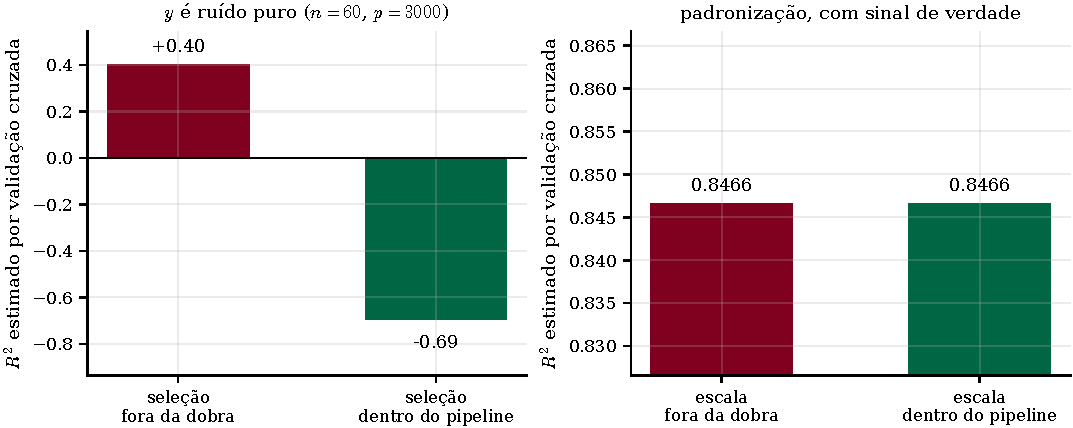
\includegraphics[width=\textwidth]{../../recursos/figuras/07-vazamento.pdf}
  \caption{Dois vazamentos, medidos em 40 repetições, com validação cruzada de 5
  dobras. \textbf{À esquerda}, seleção de variáveis: $n=60$ observações, $d=3000$
  covariáveis e uma resposta $y$ que é \emph{ruído puro}, sem nenhuma relação com
  $X$ --- o $R^2$ verdadeiro é zero. Escolher as 20 covariáveis mais correlacionadas
  com $y$ \emph{antes} da validação cruzada produz $R^2=+0{,}40$ \emph{a partir de
  nada}. Fazendo a seleção dentro do \emph{pipeline}, a CV devolve $-0{,}69$ e
  denuncia corretamente que não há sinal. \textbf{À direita}, padronização, num
  problema com sinal de verdade e escalas muito díspares: $0{,}8466$ contra
  $0{,}8466$ --- iguais até a quarta casa decimal.}
  \label{fig:vazamento}
\end{figure}

\begin{ideia}[nem todo vazamento é igual]
A lição do painel esquerdo é a que assusta: a seleção olhou $3000$ colunas de ruído
e ficou com as $20$ que, \emph{por acaso}, se pareciam com $y$ naquela amostra. As
dobras da CV vieram depois e encontraram essas 20 já escolhidas --- inclusive nas
observações que deveriam ser ``novas''. O modelo não aprendeu nada sobre o mundo;
aprendeu sobre o próprio conjunto de teste. E note que $R^2=+0{,}40$ é um número
que ninguém questionaria num relatório.

O painel direito é a lição complementar: a padronização vaza apenas duas
estatísticas robustas por coluna, calculadas sobre dezenas de observações, e a
diferença entre usar as do conjunto todo ou as do treino é numericamente
desprezível. O aviso clássico não está errado --- só não é ali que mora o perigo.
\end{ideia}

\begin{atencao}[a hierarquia que vale memorizar]
Ordenados por gravidade:
\begin{enumerate}[leftmargin=1.6cm,nosep]
  \item \textbf{Grave:} escolher variáveis, hiperparâmetros ou o próprio modelo
        olhando dados que depois serão usados para avaliar. Inflacção sem limite,
        como no painel esquerdo.
  \item \textbf{Grave:} usar informação do futuro em dados temporais, ou ter a
        mesma unidade (paciente, cliente) em treino e teste.
  \item \textbf{Leve:} padronizar, imputar pela média, codificar categóricas com o
        conjunto todo. Quase sempre inofensivo com $n$ razoável --- mas corrija
        assim mesmo, porque \textbf{custa zero}: é só pôr no \emph{pipeline}.
\end{enumerate}
\end{atencao}

%==============================================================================
\section{\emph{Pipelines}}
%==============================================================================
Um \texttt{Pipeline} encadeia etapas $(\text{nome}, \text{transformador})$
terminadas por um estimador. Ao chamar:
\begin{itemize}[leftmargin=1.4cm,nosep]
  \item \texttt{pipe.fit(X\_tr, y\_tr)}: cada transformador faz \texttt{fit\_transform}
        \emph{no treino}, em sequência, e o estimador final é ajustado;
  \item \texttt{pipe.predict(X\_te)}: cada transformador apenas \texttt{transform}
        (com os parâmetros aprendidos no treino) e o estimador prediz.
\end{itemize}
Assim, é \emph{impossível} vazar o teste por construção: o teste nunca participa de
nenhum \texttt{fit}.

\begin{figure}[htbp]
  \centering
  \begin{tikzpicture}[font=\small, x=1cm, y=1cm,
      cx/.style={draw,rounded corners=2pt,minimum height=0.62cm,inner xsep=5pt,
                 font=\footnotesize},
      seta/.style={-{Stealth[length=4pt]},gray!75}]
    % --- fluxo errado ---
    \node[font=\footnotesize\bfseries,vinho,anchor=west] at (-0.4,0.95) {errado};
    \node[cx,fill=cinzaclaro] (d1) at (0.9,0)  {dados};
    \node[cx,fill=vinho!18]   (p1) at (3.3,0)  {padroniza \emph{tudo}};
    \node[cx,fill=cinzaclaro] (s1) at (6.3,0)  {separa};
    \node[cx,fill=cinzaclaro] (a1) at (8.5,0)  {ajusta};
    \node[cx,fill=vinho!30]   (m1) at (11.2,0) {mede (otimista)};
    \foreach \a/\b in {d1/p1, p1/s1, s1/a1, a1/m1} \draw[seta] (\a) -- (\b);
    \draw[vinho,thick,-{Stealth[length=4pt]},dashed]
      (s1.south) ++(0.6,0) .. controls +(0,-0.8) and +(0,-0.8) .. (p1.south)
      node[midway,below,font=\tiny,vinho] {o teste já influenciou a média e o desvio};

    % --- fluxo certo ---
    \node[font=\footnotesize\bfseries,verdeesc,anchor=west] at (-0.4,-2.35) {certo};
    \node[cx,fill=cinzaclaro] (d2) at (0.9,-3.3)  {dados};
    \node[cx,fill=cinzaclaro] (s2) at (3.0,-3.3)  {separa};
    \node[cx,fill=verdeesc!16,draw=verdeesc,thick] (p2) at (6.3,-3.3)
        {padroniza \emph{no treino} $\to$ ajusta};
    \node[cx,fill=verdeesc!28] (m2) at (10.6,-3.3) {mede (honesto)};
    \foreach \a/\b in {d2/s2, s2/p2, p2/m2} \draw[seta] (\a) -- (\b);
    \draw[verdeesc,thick,decorate,decoration={brace,amplitude=4pt}]
      (4.75,-2.85) -- (7.85,-2.85)
      node[midway,above=3pt,font=\tiny,verdeesc] {isto é o \texttt{Pipeline}};
  \end{tikzpicture}
  \caption{A mesma análise nas duas ordens. Em cima, a padronização acontece antes
  da separação, e os parâmetros $\widehat\mu,\widehat\sigma$ carregam informação das
  observações que só deveriam aparecer na hora de medir. Embaixo, tudo o que aprende
  fica \emph{dentro} do bloco que só vê o treino --- e esse bloco é exatamente o que
  o \texttt{Pipeline} representa em código.}
  \label{fig:fluxo}
\end{figure}

\begin{lstlisting}
from sklearn.preprocessing import StandardScaler
from sklearn.linear_model import Lasso
from sklearn.pipeline import Pipeline
from sklearn.model_selection import train_test_split, GridSearchCV

X_tr, X_te, y_tr, y_te = train_test_split(X, y, test_size=0.3, random_state=0)

pipe = Pipeline(steps=[("scaler", StandardScaler()),
                       ("lasso",  Lasso())])
pipe.fit(X_tr, y_tr)        # scaler aprende mu/sigma SO do treino
pipe.predict(X_te)          # teste e apenas transformado
\end{lstlisting}

\subsection{\emph{Pipeline} $+$ validação cruzada $+$ busca de hiperparâmetros}
O grande payoff: passar o \emph{pipeline} inteiro ao \texttt{GridSearchCV}. Em cada
dobra, todo o pré-processamento é reajustado corretamente, e a busca pelos
hiperparâmetros (inclusive do scaler, se houver) fica livre de vazamento. Note a
sintaxe \texttt{nomeEtapa\_\_parametro} para acessar parâmetros de cada etapa.

\begin{lstlisting}
from sklearn.linear_model import ElasticNet

pipe_en = Pipeline([("scaler", StandardScaler()),
                    ("enet",   ElasticNet())])

param_grid = {"enet__alpha":    [0.001, 0.01, 0.1, 1, 5, 10, 50, 100],
              "enet__l1_ratio": [0.1, 0.5, 0.7, 0.9, 0.95, 0.99, 1]}

busca = GridSearchCV(pipe_en, param_grid, cv=5,
                     scoring="neg_mean_squared_error")
busca.fit(X_tr, y_tr)               # CV SEM vazamento, etapa por etapa
print("melhores parametros:", busca.best_params_)
print("risco no teste:", -busca.score(X_te, y_te))
\end{lstlisting}

\begin{atencao}
Repare que a última linha usa \texttt{X\_te}, que o \texttt{GridSearchCV} nunca
viu. Isso é obrigatório: o \texttt{busca.best\_score\_} é o melhor resultado
\emph{de $56$ combinações testadas}, e o máximo de 56 estimativas ruidosas é
otimista por construção --- mesmo com a CV feita corretamente. É a validação
aninhada da Aula~03, na prática: a CV escolhe, o teste mede.
\end{atencao}

\begin{ideia}
Encare o \emph{pipeline} como ``o modelo''. Tudo o que você faria errado à mão ---
padronizar cedo demais, esquecer de aplicar a mesma transformação no teste, vazar
na CV --- o \emph{pipeline} previne por construção. É a tradução em código das regras
das Aulas~02--04.
\end{ideia}

%==============================================================================
\section{Outros pré-processamentos comuns}
%==============================================================================
\begin{description}[leftmargin=2.6cm,style=nextline]
  \item[Imputação] preencher valores faltantes (\texttt{SimpleImputer} com média,
        mediana ou moda). A estatística de imputação também se aprende \emph{só no
        treino}.
  \item[Codificação de categóricas] \texttt{OneHotEncoder} (cria \emph{dummies}) ou
        \texttt{OrdinalEncoder}. Lembre (Aula~06) que árvores lidam com categóricas
        sem isso. Use \texttt{handle\_unknown="ignore"}: uma categoria pode existir
        no teste e não no treino, e sem isso o \texttt{predict} quebra.
  \item[Escalas alternativas] \texttt{MinMaxScaler} (intervalo $[0,1]$),
        \texttt{RobustScaler} (baseado em quantis, resistente a \emph{outliers}).
  \item[Redução de dimensão] PCA como etapa do \emph{pipeline} (Aula extra E2),
        também ajustado apenas no treino. Ele aprende direções de todas as colunas
        ao mesmo tempo, o que parece grave --- mas \textbf{não olha o $Y$}, e por
        isso não consegue fabricar sinal a partir de ruído: a medição da Aula~E2 o
        coloca na categoria \emph{leve} desta hierarquia, junto com a padronização.
\end{description}

Quando diferentes colunas precisam de tratamentos diferentes (numéricas
padronizadas, categóricas codificadas), usa-se o \texttt{ColumnTransformer}:
\begin{lstlisting}
from sklearn.compose import ColumnTransformer
from sklearn.preprocessing import OneHotEncoder, StandardScaler
from sklearn.impute import SimpleImputer

prep = ColumnTransformer([
    ("num", Pipeline([("imp", SimpleImputer(strategy="median")),
                      ("sc",  StandardScaler())]), colunas_numericas),
    ("cat", OneHotEncoder(handle_unknown="ignore"), colunas_categoricas),
])
modelo = Pipeline([("prep", prep), ("clf", Lasso())])
\end{lstlisting}
Note que o \texttt{ColumnTransformer} é, ele próprio, uma etapa de um
\emph{pipeline} maior, e que a coluna numérica passa por um \emph{pipeline}
aninhado. A estrutura é recursiva de propósito: qualquer análise, por mais
complicada, cabe num único objeto com um \texttt{fit} e um \texttt{predict}.

O notebook \texttt{Aula prática 07} monta esse fluxo completo, reproduz as duas
medições da Figura~\ref{fig:vazamento} e acrescenta uma terceira: o vazamento por
observações agrupadas, que nenhum \emph{pipeline} evita.

%==============================================================================
\section*{Resumo}
%==============================================================================
\begin{itemize}[leftmargin=1.4cm]
  \item Pré-processamento que aprende parâmetros é \textbf{parte do modelo}: ajuste
        só no treino, aplique ao teste (Fig.~\ref{fig:fluxo}).
  \item \textbf{Padronização} \eqref{eq:std}: adimensionaliza, equaliza escalas
        (essencial para KNN e penalização, irrelevante para árvores), dispensa
        intercepto; custo: leve perda de interpretabilidade.
  \item \textbf{Vazamento} não é tudo igual (Fig.~\ref{fig:vazamento}): seleção de
        variáveis ou de hiperparâmetros fora da dobra fabrica $R^2$ do nada;
        padronizar fora da dobra é, na prática, quase inofensivo. Corrija os dois
        --- o \emph{pipeline} torna isso gratuito.
  \item \textbf{\emph{Pipeline}}: encadeia tudo num único objeto e previne
        vazamento por construção; combine com \texttt{GridSearchCV} e ainda assim
        meça no teste.
  \item \texttt{ColumnTransformer} aplica tratamentos distintos a colunas distintas,
        e aninha \emph{pipelines} dentro de \emph{pipelines}.
\end{itemize}

\paragraph{Leitura recomendada.} [ISLP] laboratórios dos Capítulos~5 e~6, onde os
autores montam exatamente esses fluxos em Python; [AME] §2.1.2 (regressão linear na
prática). Documentação do \texttt{scikit-learn}: \emph{Pipelines and composite
estimators} e \emph{Common pitfalls and recommended practices}, esta última dedicada
ao vazamento. Para o experimento da Figura~\ref{fig:vazamento}, o texto de
referência é Hastie, Tibshirani \& Friedman, \emph{The Elements of Statistical
Learning}, §7.10.2 (``The Wrong and Right Way to Do Cross-validation'').

\paragraph{Para praticar.} \texttt{recursos/listas/Lista de exercícios 07.pdf}.

\end{document}
